\begin{frame}
\begin{itemize}
    \item \textbf{\color{red}{What are Normalizing Flows}}
    \item NICE
    \item RealNVP
    \item GLOW
    \item GamePlan
    \item Results
\end{itemize}
\end{frame}

\begin{frame}
    \frametitle{What are Normalizing Flows?}
    \begin{itemize}
        \item Generative models, like GANs and VAEs.  \footnote{Source:
    https://lilianweng.github.io/lil-log/2018/10/13/flow-based-deep-generative-models.html}
        \item Gets \textbf{explicit} representation of density function (GANs
            and VAEs get implicit).
        \item Sequence of invertible transformations (e.g. $f(x) = \sigma x +
            \mu$ and $f^{-1}(x) = \sigma x - \mu$)
    \end{itemize}
    \center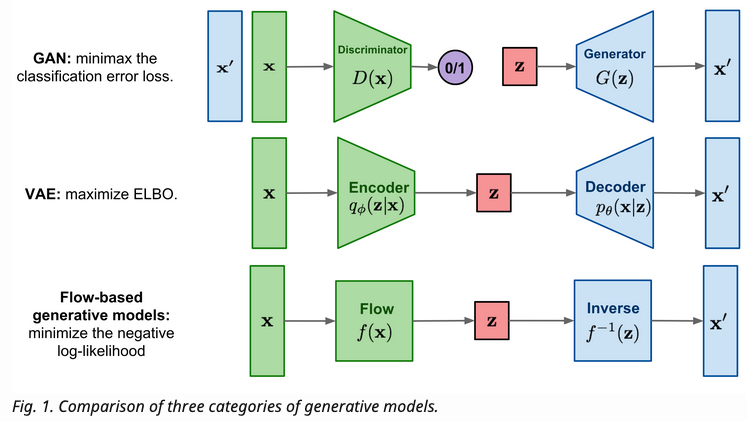
\includegraphics[width=0.75\textwidth]{GenerativeModels.png}
\end{frame}

\begin{frame}
    \frametitle{What are Normalizing Flows? (Steven)}
    \center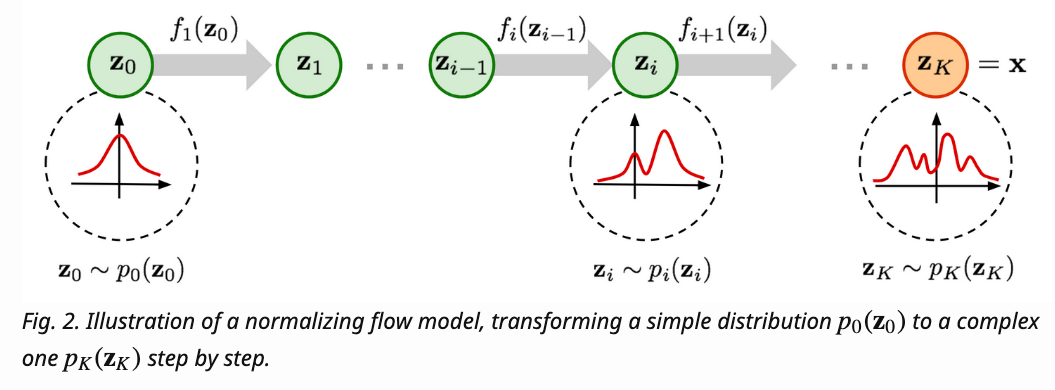
\includegraphics[width=0.95\textwidth]{NFs.png}
\end{frame}

\begin{frame}
    \frametitle{What are Normalizing Flows?}
    We rely on Change of Variables in probailty distributions. Let
    $\mathbf{z}\in \mathbb{R}^d$ be a random variable and a mapping function $f:
    \mathbb{R}^d \mapsto \mathbb{R}^d$. We can use $f$ to transform
    $\mathbf{z}\sim q(\mathbf{z})$ and get a random variable $\mathbf{y} =
    f(\mathbf{z})$ and the following probability distribution
    \[
        q_y(\mathbf{y}) = q(\mathbf{z})\left | det(\frac{\partial
        f}{\partial \mathbf{z}}) \right | ^{-1}
    \]
    if we diagonalize our jacobian we can make the determinant easier to solve
    and make our transformation dependent on less variables. 
    \begin{align*}
        y_1 &= T_1(z_1)\sim q_1(y_1)\\
        y_2 &= T_2(z_1,z_2)\sim q_2(y_2 | y_1)\\
        y_3 &= T_3(z_1,z_2,z_3)\sim q_3(y_3|y_1,y_2)\\
        y_n &= T_n(z_1,\dots,z_n)\sim q_n(y_n|y_1,\dots,y_{n-1})
    \end{align*}

\end{frame}

\begin{frame}
    \frametitle{What are Normalizing Flows?}
    \begin{itemize}
        \item Can get sharp images with log-liklihood (goodness of fit).
        \item Can explore latent space and generate different modes (e.g. We can
            turn a person old if we know where old people are in the
            distribution)
    \end{itemize}
    \pause
    But
    \begin{itemize}
        \item Need determinant of Jacobian (use LU Decomposition to make
            faster)
        \item Need \textbf{lots} of data for high dimensional problems.
    \end{itemize}
\end{frame}

